\documentclass[letter]{article}
\renewcommand{\baselinestretch}{1.25}

\usepackage[margin=1in]{geometry}
\usepackage{physics}
\usepackage{amsmath}
\usepackage{graphicx}
\usepackage{hyperref}


% MATLAB Formating Code
\usepackage[numbered,framed]{matlab-prettifier}
\lstset{style=Matlab-editor,columns=fullflexible}
\renewcommand{\lstlistingname}{Script}
\newcommand{\scriptname}{\lstlistingname}



% Document Specific
\newcommand{\sat}{\text{sat}}


\allowdisplaybreaks

%opening
\title{MECH 6313 - Homework 4}
\author{Jonas Wagner}
\date{2021, March 26}

\begin{document}

\maketitle


\section{Problem 1}

\subsection{Part a}
\textbf{Problem:}
Let the plant $$\frac{1}{s^2}$$ be defined with no input and the following state-space representation: 
\begin{equation}
	\begin{aligned}
		\dot{x}_1 &= x_2\\
		\dot{x}_2 &= 0
	\end{aligned}
\end{equation}
What can be said about the equilibrium stability of the system?\\

\noindent
\textbf{Solution:}
The defined system is a linear system with now input defined with $$A = \mqty[0&1\\0&0]$$
From this it is clear that their exists a single Jordan block with two poles at $\lambda_{1,2} = 0$.

The system is therefore unstable as the multiplicity of the roots are on the $j\omega$-axis is greater then one which disqualifies the system from marginal stability.

%\newpage
\subsection{Part b}
\textbf{Problem:}
Let the magnetically suspended ball system be defined as
\begin{equation}
	\begin{aligned}
		\dot{x}_1 &= x_2\\
		\dot{x}_2 &= \cfrac{-c \bar{u}^2}{m x_1^2} + g
	\end{aligned}
\end{equation}
with the input $$\bar{u}= \sqrt{\frac{mg}{c}Y}$$ defined as a constant.

What can be said about the stability of the system at it's equilibrium?\\

\noindent
\textbf{Solution:}
The equilibrium points of the system can be found by solving for the points where the state equations are equal to zero.
It is clear that all equilibrium points occur when $\dot{x}_2 = 0$.

\begin{align}
	\dot{x}_2 = 0 &= \cfrac{-c \bar{u}^2}{m x_1^2} + g\\
	\cfrac{c \bar{u}^2}{m x_1^2} &= g\\
	c \bar{u}^2 &= mg x_1^2\\
	x_1^2 &= \cfrac{c \bar{u}^2}{mg}\\
	x_1 &= \sqrt{\cfrac{c \bar{u}^2}{mg}}
	\intertext{By substituting the defined steady-state input, the following can be obtained:}
	x_1 &= \sqrt{\cfrac{c \sqrt{\frac{mg}{c}Y}^2}{mg}} = \sqrt{Y}
\end{align}
Thus the equilibrium point is at
\begin{equation}
	\begin{aligned}
		x_1 &= \sqrt{Y}\\
		x_2 &= 0
	\end{aligned}
\end{equation}

The linearization of the system can then be obtained by evaluating the jacobian matrix at the equilibrium point:
\begin{align}
	A 	&= \eval{\mqty[	0 & 1\\
			\cfrac{2 c \bar{u}^2}{m x_1^3} &0]}_{x_1 = \sqrt{Y}, \ x_2 = 0}\\
		&= \mqty[0 & 1\\
				\cfrac{2 c \sqrt{\frac{mg}{c}Y}^2}{m \sqrt{Y}^3} &0]
	\intertext{Which can be simplified into the linear dynamics defined by the A matrix:}
	A	&= \mqty[0 & 1\\ \cfrac{2g}{\sqrt{Y}} & 0]
\end{align}
This system linearization around the equilibrium point can be analyzed to see that the characteristic polynomial is $$s^2 - \cfrac{2g}{\sqrt{Y}}$$
The poles of the linearized system can then be found as $$\lambda_{1,2} = \pm \sqrt{\cfrac{2g}{\sqrt{Y}}} = \pm \cfrac{\sqrt{2g}}{\sqrt[4]{Y}} = \pm \sqrt{2g} \ \qty(Y)^{-\frac{1}{4}}$$
From this it can be seen that the system is unstable at the equilibrium point due to the positive pole at $\lambda_1 = \sqrt{2g}(Y)^{\frac{1}{4}}$.

\newpage
\section{Problem 2}
An unforced morse oscilator is governed by the following equations:
\begin{equation}
	\begin{aligned}
		\dot{x}_1 &= x_2\\
		\dot{x}_2 &= - \mu \qty(e^{-x_1} - e^{-2x_1})
	\end{aligned}
\end{equation}

\subsection{Part a}
\textbf{Problem:}
Find the equalibrium points of the system.

\noindent
\textbf{Solution:}
The equilibrium points of the system can be found by solving for the points where the state equations are equal to zero.
It is clear that all equilibrium points occur when $\dot{x}_2 = 0$.

\begin{align}
	\dot{x}_2 = 0 &= - \mu \qty(e^{-x_1} - e^{-2x_1})\\
	-\mu e^{-x_1} &= e -\mu e^{-2x_1}\\
	-x_1 &= -2x_1\\
	x_1 &= 0
\end{align}

Thus, the only equilibrium point occurs at the origin.

\subsection{Part b}
\textbf{Problem:}
Assess the stability properties of the equilibrium point.

\noindent
\textbf{Solution:}
Linearization of the model around the origin produces the following dynamic matrix:
\begin{equation}
	A = \mqty[	0 & 1\\
				-\mu & 0]
\end{equation}
The associated characteristic polynomial is given as $$s^2 + \mu$$ thus the eigenvalues of the system are $$\lambda_{1,2} = \pm j \sqrt{\mu}$$
From this it can be said that the linearized system in marginally stable as the roots of the system are purely imaginary. However this does not explicitly provide that the nonlinear system is stable.

The alternative method of proving this marginal stability is to directly use a Lyapnov Function defined by
\begin{equation}
	V(x) = \frac{1}{2} x_2^2 + \int_0^{x_1} \mu \qty(e^{-\xi} + e^{-2\xi}) \dd \xi
\end{equation}
and show the negative semi-definess of $\dot{V}(x)$:
\begin{align}
	\dot{V}(x) &= x_2 \dot{x}_2 + \mu \qty(e^{-x_1} + e^{-2x_1}) \dot{x}_1\\
	&= x_2 \qty(- \mu \qty(e^{-x_1} - e^{-2x_1})) + \mu \qty(e^{-x_1} + e^{-2x_1}) \qty(x_2)\\
	&= 0 \leq 0
\end{align}
thus the system is shown to be stable in the sense of lyapnov (marginally stable).






\newpage
\section{Problem 3}
A nonlinear system is given as
\begin{equation}
	\begin{aligned}
		\dot{x}_1 &= x_2\\
		\dot{x}_2 &= -g \qty(k_1 x_1 + k_2 x_2), \ k_1, k_2 > 0
	\end{aligned}
\end{equation}
where $g(\cdot)$ is known to satisfy the following
\begin{equation}
	\begin{aligned}
		y g(y) > 0, \ \forall y \neq 0\\
		\lim_{\abs{y} \to \infty} \int_0^y g(\xi) \dd{\xi}  = + \infty
	\end{aligned}
\end{equation}

\subsection{Part a}
\textbf{Problem:}
Use an appropriate lyapnov function to show that the equilibrium point at $x=0$ is globally asymptotically stable.

\noindent
\textbf{Solution:}
Let,
\begin{equation}
	V(x) = \int_0^{x_1} g(\xi) \dd \xi + \frac{1}{2} x_2^2
\end{equation}
which is a viable Lyapnov function candidate. The derivative can then be found as
\begin{align}
	\dot{V}(x) &= g(x_1) \dot{x_1} + x_2 \dot{x}_2\\
	&= g(x_1) x_2 + x_2 (-g(k_1 x_2 + k_2 x_2))\\
	\intertext{taking an mild superposition assumption with the stipluation that sign is critical, but magnitudes are still iffy,}
	&\leq x_2 g(x_1) - x_2 g(k_1 x_2) - x_2 g(k_2 x_2)\\
	\intertext{from the definition of the $g(\cdot)$ function, the following can also be derived}
	&\leq - x_2 g(k_2 x_2) < 0
\end{align}
Therefore, $\dot{V}(x)$ is strictly negative definite and thus the system is known to be globally asymptotically stable.

\newpage
\subsection{Part b}
\textbf{Problem:}
Show that the saturation function $$\text{sat}(y) = \text{sign}(y) \min \{1, \abs{y}\}$$ satisfies the above assumptions for $g(\cdot)$.

What is the exact form of your Lyapnov function for this saturation nonlinearity?\\

\noindent
\textbf{Solution:}
The conditions for $g(y)$ can be satisfied for the positive and negative domains to prove that $\text{sat}(y)$ satisfies the conditions $\forall x \neq 0$.\\

First, for $y > 0$,
\begin{align}
	y \sat(y) &= y \ \text{sign} \min{1,\abs{y}}\\
	&= (+1) \abs{y} (+1) (+K), \ K = \min{1,\abs{y}}\\
	&> 0, \forall y > 0
\end{align}
and the other condition is also easily demonstrated
\begin{align}
	\lim_{\abs{y} \to \infty} \int_0^y \sat(\xi) \dd{\xi} 
	&= \lim_{y \to \infty} \int_0^y (+1) (+ K) \dd{\xi}, \ K = \min{1,\xi}\\
	&= + \infty
\end{align}


Second, for $y < 0$,
\begin{align}
	y \sat(y) &= y \ \text{sign} \min{1,\abs{y}}\\
	&= (-1) \abs{y} (-1) (+K), \ K = \min{1,\abs{y}}\\
	&> 0, \forall y > 0
\end{align}
and the other condition is also easily demonstrated
\begin{align}
	\lim_{\abs{y} \to \infty} \int_0^y \sat(\xi) \dd{\xi} 
	&=\lim_{y \to - \infty} \int_0^y (-1) (+ K) \dd{\xi}, \ K = \min{1,\xi}\\
	&= \lim_{y \to - \infty} - \int_y^0 (-1) (+ K) \dd{\xi}, \ K = \min{1,\xi}\\
	&= + \infty
\end{align}

Thus, $\sat{y}$ satisfies all the conditions of a $g(\cdot)$ function.

From this, and the intuition around $g(y)$ functions, we can then conclude that the system (when controlled as stated) the saturated system is globally asymptotically stable. Specifically a Lyapnov function of the form $V(y) = y \sat(y)$ could be used.

\newpage
\subsection{Part c}
\textbf{Problem:}
Demonstrate that a double integrator with a saturation actuator, given as
\begin{equation}
	\begin{aligned}
		\dot{x}_1 &= x_2\\
		\dot{x}_2 &= \text{sat}(u)
	\end{aligned}
\end{equation}
can be saturated with the state-feedback controller $$ u = -k_1 x_1 - k_2 x_2$$ and design $k_1$ and $k_2$ such that the eigenvalues of the linearization are placed at $\lambda_{1,2} = -1 \pm j$.

Simulate the closed loop with and without saturation and compare the resulting trajectories vs time.

\noindent
\textbf{Solution:}
MATLAB and Simulink were used to calculate gains as well as simulate the stabilization of the saturated double integrator system.

The negative feedback controller gains to achieve the desired poles was calculated to be:
\begin{equation}
	K = \mqty[2 & 2]
\end{equation}

The simulink model that was used to simulate consisted of an LTI system representing the double integrator, a saturation block, and a gain for feedback. The model can be seen in \figurename \ \ref{fig:pblm3_c_model}. 
\begin{figure}[h]
	\centering
	\label{fig:pblm3_c_model}
	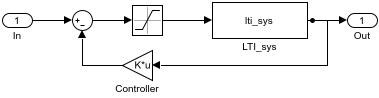
\includegraphics[width=0.5\textwidth]{fig/pblm3_c_model}
	\caption{Simulink model used to simulate the saturated double integrator.}
\end{figure}

The results for stabilization of the system with initial conditions $x_0 = \mqty[1 &-1]^T$ is shown in \figurename \ \ref{fig:pblm3_c_plot}.
\begin{figure}[h]
	\centering
	\label{fig:pblm3_c_plot}
	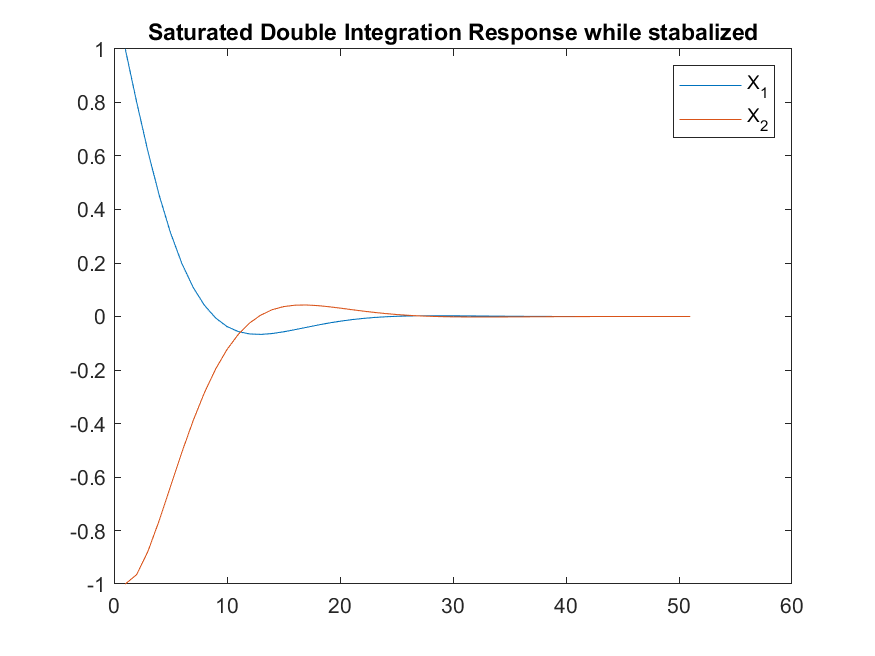
\includegraphics[width=0.5\textwidth]{fig/pblm3_c_plot}
	\caption{Simulation results of the stabilization of the saturated double integrator.}
\end{figure}









\newpage
\section{Problem 4: K4.14}
A nonlinear system is given as
\begin{equation}\label{eq:pblm4_sys}
	\begin{aligned}
		\dot{x}_1 &= x_2\\
		\dot{x}_2 &= -g(x_1) (x_1 + x_2)
	\end{aligned}
\end{equation}
where $g(\cdot)$ is known to be locally Lipschitz continuous and satisfies $g(y) \geq 1, \ \forall y \in \real$.

\noindent
\textbf{Problem:}
Verify that
\begin{equation}
	V(x) = \int_0^{x_1} y g(y) \dd{y} + x_1 x_2 + x_2^2
\end{equation}
is positive  definite $\forall \ x \in \real^2$ and radially unbounded. Next use $V(x)$ to shown that $x=0$ is globally asymptotically stable.\\

\noindent
\textbf{Solution:}
To prove that (i) $V(x)$ is positive definite, it must be true that $V(0) = 0$ and (ii) $V(x) > 0 \ \forall x \in \{ \real^2 \backslash (0,0)\}$. First, (i) can be shown as:
\begin{align}
	\eval{V(x)}_0 = 0
	&= \eval{\qty(\int_0^{x_1} y g(y) \dd{y} + x_1 x_2 + x_2^2)}_0\\
	&= \int_0^{0} y g(y) \dd{y} + (0)(0) + (0)^2\\
	&= 0
\end{align}

(ii) can then be shown by first demonstrating that since $g(y) \geq 1, \ \forall y \in \real$, the following is true
\begin{align}
	\int_0^{x_1} y g(y) \dd{y}
	&\geq \int_0^{x_1} y (1) \dd{y}\\
	&\geq \frac{1}{2} x_1^2\\
	&\geq 0, \ x_1 \neq 0
\end{align}
additionally, it is obvious that $$x_2^2 \geq 0, \ x_1 \neq 0$$
and the following statements are also true
\begin{align}
	x_1 x_2 &\geq 0, \ x \in \{x_1, x_2 \geq 0\} \bigcup \{x_1, x_2 \leq 0\}\\
	\abs{x_1 x_2} &< \frac{1}{2} x_1^2 + x_2^2, \ x \in \{x_1 < 0, x_2 > 0\} \bigcup \{x_1 > 0, \ x_2 < 0\}
\end{align}
The following therefore true
\begin{align}
	V(x) &\geq \frac{1}{2} x_1^2 + x_1 x_2 + x_2^2 \geq 0
\end{align}
Thus $V(x) \succ 0$ and is clearly radially unbounded as the lyapnov function is defined over the entire domain $x \in \real^2$.

\newpage
The lyapnov function can now be used to demonstrate that \eqref{eq:pblm4_sys} is globally asymptotically stable by the following:
\begin{align}
	\dot{V} = \dv{V}{x} \dv{x}{t}
	&= \qty(x_1 g(x_1) + x_2) \dot{x}_1 + \qty(x_1 + 2 x_2) \dot{x}_2\\
	&= \qty(x_1 g(x_1) + x_2) \qty(x_2) + \qty(x_1 + 2 x_2) \qty(-g(x_1) \qty(x_1 + x_2))\\
	&= x_1 x_2 g(x_1) + x_2^2 - x_1^2 g(x_1) - x_1 x_2 g(x_1) -2 x_1 x_2 g(x_1) -2 x_2^2 g(x_1)\\
	&= x_2^2 -g(x_1) \qty(x_1^2 + 2 x_1 x_2 + 2 x_2^2)
	\intertext{since $g(y) \geq 1, \ \forall y \in \real$,}
	&\leq x_2^2 - \qty(x_1^2 + 2 x_1 x_2 + 2 x_2^2)\\
	&\leq -x_1^2 - 2x_1 x_2 - x_2^2\\
	&\leq - (x_1 + x_2)^2 < 0, \ x_1, x_2 \neq 0
\end{align}
Therefore, $\dot{V}(x) \prec 0$ and the system is globally asymptotically stable.











\newpage
\appendix
\section{MATLAB Code:}\label{apx:matlab}
All code I write in this course can be found on my GitHub repository:\\
\href{https://github.com/jonaswagner2826/MECH6313}{https://github.com/jonaswagner2826/MECH6313}
% MECH6313_HW3
\lstinputlisting[caption={MECH6313\_HW4},label={script:HW4}]{MECH6313_HW4.m}


\end{document}
